\documentclass[unicode,review]{siamart1116}

\usepackage{color}
\usepackage{amsmath}
\usepackage{amsfonts}
\usepackage{amssymb}
\usepackage{mathabx}
\usepackage{geometry}
\usepackage{graphicx}
\usepackage{pgf}
% May be removed later
\usepackage{todonotes}

\newcommand{\llinnm}[2]{\operatorname{L}_{\operatorname{lin}}({#1}, {#2})}
\newcommand{\llinn}[1]{\llinnm{#1}{#1}}
\newcommand{\hlinr}[1]{\operatorname{H}_{\operatorname{lin}}^{#1}}
\newcommand{\hlin}{\operatorname{H}_{\operatorname{lin}}}
\newcommand{\leap}[3]{\operatorname{\mathbf{leap}}({#1}, {#2}, {#3})}
\newcommand{\hfact}[2]{\operatorname{H}_{\operatorname{factor}}({#1}, {#2})}
\newcommand{\rot}[2]{\operatorname{H}_{\operatorname{rot}}^{{#1}, {#2}}}

\newcommand{\bin}[3]{\operatorname{\mathbf{bin}}({#1}, {#2}, {#3})}
\newcommand{\lbin}[2]{\operatorname{\mathbf{lbin}}({#1}, {#2})}

\newcommand{\vecspace}[2]{\mathbb{Z}_{#1}^{#2}}
\newcommand{\binvecspace}[1]{\vecspace{2}{#1}}
\newcommand{\linearmaps}[2]{\mathcal{L}_{#1}^{#2}}
\newcommand{\surjectivelinearmaps}[2]{\mathcal{LS}_{#1}^{#2}}

\newcommand{\probs}[2]{\operatorname{\mathbf{Pr}}_{{#1}}\left[{#2}\right]}
\newcommand{\prob}[1]{\probs{}{#1}}
\newcommand{\expects}[2]{\operatorname{\mathbf{E}}_{{#1}}\left[{#2}\right]}
\newcommand{\expect}[1]{\expects{}{#1}}
\newcommand{\inu}{\in_U}

\newtheorem{claim}{Claim}

% SIAM template
\numberwithin{theorem}{section}

\newcommand{\TheTitle}{On the Size of Largest Bins Using Placement with Linear
Transformations} 
\newcommand{\TheAuthors}{M. Babka}

\title{\TheTitle}

\headers{\TheTitle}{\TheAuthors}

\author{
  Martin Babka\thanks{Charles University, Prague (\email{babkys@gmail.com}).}
}

\usepackage{amsopn}
\DeclareMathOperator{\diag}{diag}

\ifpdf
\hypersetup{
  pdftitle={\TheTitle},
  pdfauthor={\TheAuthors}
}
\fi
% End SIAM template
\begin{document}

\maketitle

\begin{abstract}
We are studying placement of $n$ balls into $n$ bins where balls and bins are represented as two vector spaces over $\binvecspace{2}$. The placements is done according a linear transformation between the two vector spaces.
We analyze the expected size of the largest bin. The only currently known upper bound is is $O(\log n \log \log n)$ by Alon et al. and holds for placing $n \log n$ balls into $n$ bins.
We show that this bound can be improved to $O(\log n)$ in the case when $n$ balls are placed into $n$ bins.
We reuse the same technique as it is in the article by Alon et al. but switch to a different parametrization of the building blocks.
\end{abstract}

\begin{keywords}
balls and bins, universal hashing, linear transformations
\end{keywords}

\begin{AMS}
  68W20, % Randomized algorithms
  68P05, % Data structures
  68W40  % Analysis of algorithms
\end{AMS}

\section{Introduction}

Research of hash function families is nowadays naturally focused on finding fast systems suitable for universal hashing, cuckoo hashing, linear probing, load balancing, etc.
Each application has slightly different requirements on the used system.
For example universal hashing~\cite{cw} requires families having small largest bins, for linear probing we have to to provide a 5-independent family~\cite{linear-probing}.
And not only the mentioned requirements have to be fulfilled yet the time to compute a function should be small.

In this article we are dealing with the size of a largest bin in a special balls-and-bins setting.
It is known that if we randomly and independently place $n$ balls into $n$ bins, then the size of a largest bin is $\Theta(\log n/\log \log n)$ with high probability.
This bound can be achieved by various systems, especially by completely independent uniform placement, by systems constructed in \cite{siegel} and \cite{celisetal}. 
Let us note that relaxing full independence to $\log n/\log \log n$-independence is also possible without asymptotically worsening the above bound.
Hash function families with high degrees of independence provide perfect results for many other applications e.g. as concentration bounds.

Unfortunately the systems with high independence are inefficient in practice because of size and/or speed according to Siegel's lower bound~\cite{siegel}. 
The research then moved from finding highly independent systems to finding functions which best fit the needs of the application. 
As already mentioned efficient systems specially designed to achieve the optimal bound of balls-and-bins emerged in \cite{celisetal}.
There are also special designs of hash function systems which accommodate to the special needs of the settings required by cuckoo hashing, linear probing, etc.
For cuckoo hashing there are known families and modifications of the scheme which keep the expected $O(1)$ operation time such as cuckoo hashing with stash from \cite{mitzenmacher-cuckoo} and \cite{dietzfelbinger-cuckoo}.
For linear probing it is known that 5-indepence is enough to achieve the expected constant probe sequence length~\cite{linear-probing}.

The system of linear transformations between the binary vector spaces forms a simple and natural two-wise independent system of functions.
We show that this system achieves the size of a largest bin which is nearly optimal despite its only 2-independence.
We assume that $n = 2^b$ and we have $n$ elements arbitrarily chosen from the universe, the vector space $\binvecspace{u}$.
We show that if $n$ balls are placed into the table of size $n$ using a randomly chosen linear transformation from $\binvecspace{u}$ to $\binvecspace{b}$, then the expected size of a largest bin is $O(\log n)$.
It has been already shown in a paper by Alon et al \cite{alonetal} that the bound achieved by linear transformations is $O(\log n \log \log n)$ for placing $n \log n$ balls into $n$ bins.
This bound certainly holds for placing $n$ balls into $n$ bins.
We improve the previous bound by $\log \log n$ factor when assuming that just $n$ balls are placed into the same number of bins.

The technique of the proof is similar as in the original proof. 
We switch to a different parametrization and change a few statements so that they suit the current setting.
Our result was still not known and published and the asymptotic improvement has impact on universal hashing using this family of functions.
The dictionary problem solved by universal hashing with linear transformations has now expected ``worst case'' guarantee which matches the running times achieved by balanced trees.

\section{Notation and the setting}
Let $u, b \in \mathbb{N}$ and $A$ be a binary matrix of dimension $u \times b$, i.e. $A \in \{0, 1\}^{u \times b}$, and $\vec{a} \in \binvecspace{b}$. 
By affine linear transformation from $\binvecspace{u}$ to $\binvecspace{b}$ we understand a mapping $x \mapsto Ax + \vec{a}$.
By linear transformation from $\binvecspace{u}$ to $\binvecspace{b}$
we understand a mapping $x \mapsto Ax$, i.e. affine transformation with $\vec{a} = \vec{0}$.
Notice that the choice of $\vec{a}$ does not change the bin sizes and thus for placing balls into bins we may use linear transformations only.

By $\linearmaps{u}{b}$ we denote all linear transformations from $\binvecspace{u}$ to $\binvecspace{b}$.
By $\surjectivelinearmaps{u}{b}$ we denote all surjective linear transformations from $\binvecspace{u}$ onto $\binvecspace{b}$.
Let $S \subseteq \binvecspace{u}$ and $T \in \linearmaps{u}{b}$, then by $\lbin{T}{S}$ we denote the size of a largest bin created by $T$ when hashing $S$, i.e. $\lbin{T}{S} = \operatorname{argmax}_{y \in \binvecspace{b}} |T^{-1}(y) \cap S|$.

When considering probability of an event $E$ or the expected value of a variable $V$ we use $\probs{h \in_U H}{E}$ or $\expects{h \in_U H}{V}$ to indicate that the probability space is formed by random uniform choice of an object $h$ from a set $H$.

\section{Placement of \texorpdfstring{$n$}{n} Balls into \texorpdfstring{$n$}{n} Bins}

Throughout this section we assume the placement of $n$ balls into $n$ bins using linear transformations.
Moreover we assume that $n = 2^b$ for a positive integer $b$.
The universe is $\binvecspace{u}$ and the stored set is $S \subseteq \binvecspace{u}$ with $|S| = n$.
\begin{theorem}
\label{theorem-n-to-n}
Let $S \subseteq \binvecspace{u}$ and let $n = |S|$. It holds that $\expects{T \in_U \linearmaps{u}{\log n}}{\lbin{T}{S}} = O(\log n)$.
\end{theorem}
To prove \cref{theorem-n-to-n} we proceeded in the same way as it is done to prove $\log n \log \log n$ bound for placement of $n \log n$ balls into $n$ bins in \cite{alonetal}.
We cite all the old and provide the proofs of all the new claims.
The main difference between the two approaches is switching to a different parametrization which better suits our case.
We cite the results proved in \cite{alonetal} that are directly reused.
\begin{theorem}
\label{theorem-prob-bound}
Let $t, u \in \mathbb{N}$, $t < u$.
Let $S \subseteq \binvecspace{u}$ such that $\alpha = 1 - \frac{|S|}{2^u}$, $\alpha < 1$.
Then 
\[
\probs{T \in_U \surjectivelinearmaps{u}{t}}{T(S) \neq \binvecspace{t}} \leq \alpha^{u - t - \log t + \log \log \frac{1}{\alpha}}.
\]
\end{theorem}
\begin{proof}
Theorem~{7b} from \cite{alonetal}.
\end{proof}

\begin{theorem}
\label{theorem-epsilon}
Let $t \in \mathbb{N}$.
Then for each $\epsilon > 0$ exists $c_\epsilon > 0$ such that for each $S \subset \binvecspace{u}$, $|S| \geq c_\epsilon t 2^t$ it holds  $\probs{T \in_U \linearmaps{u}{t}}{T(S) = \binvecspace{t}} \geq 1 - \epsilon$.
\end{theorem}
\begin{proof}
Theorem~{7a} from \cite{alonetal}.
\end{proof}

We now define two events needed to estimate the probability of having a large bin. 
Both of them originally appeared in \cite{alonetal}.
The first event, $E_1$, occurs iff there is a bin of size at least $l$.
The second one, $E_2$ is used to bound the probability of occurrence of  $E_1$.
\begin{definition}[Event $E_1$]
Let $l \in \mathbb{N}$, $T \in \linearmaps{u}{b}$. We define $E_1(S, T, l)$ as $\exists \vec{y} \in \binvecspace{b} \colon |T^{-1}(y) \cap S| \geq l$.
\end{definition}

To define the second event, $E_2$, we factor the chosen random linear map $T \in \linearmaps{u}{b}$ through a factor vector space $\binvecspace{f}$ into two linear maps.
We factor $T$ into $T_0 \in \linearmaps{u}{f}$ and a surjective $T_1 \in \surjectivelinearmaps{f}{b}$ satisfying that $T = T_0 \circ T_1$.

\begin{definition}[Event $E_2$]
Let $u, f, b \in \mathbb{N}$, $f \geq b$, $S \subseteq \binvecspace{u}$, $T_0 \in \linearmaps{u}{f}$ and $T_1 \in \surjectivelinearmaps{f}{b}$.
The event $E_2(S, T_0, T_1)$ occurs when $\exists \vec{y} \in \binvecspace{b} \colon T_1^{-1}(y) \subseteq T_0(S)$.
\end{definition}

From now on we reserve the following symbols for the factorization; we assume that $u, f, b \in \mathbb{N}$, $f \geq b$, $S \subseteq \binvecspace{u}$, $T_0 \in_U \linearmaps{u}{f}$ and $T_1 \in_U \surjectivelinearmaps{f}{b}$ and $T = T_0 \circ T_1$.

The event $E_2$ co-occurs along with $E_1$ with at least a constant probability as is analyzed in \cref{lemma-e1-e2}. 
Using this fact we may bound the probability of $E_1$ by bounding the probability of occurrence of $E_2$ as it is in \cref{corollary-e1-e2} of \cref{lemma-e1-e2}.
Let us note that the proofs of the lemma and the corollary come from~\cite{alonetal}.
On the other hand we proceed more slowly and provide more formal statements.
We also explicitly consider the probabilities along with their probability spaces.

\begin{lemma}
\label{lemma-e1-e2}
Assume that the linear mappings $T, T_1$ are fixed.
Also assume that the linear mapping $T_0$ is fixed so that $T = T_0 \circ T_1$ except for its part $T_k$. $T_k$ is a linear mapping which maps the kernel of $T$ to the kernel of $T_1$.
For each $\epsilon > 0$ there is $c_\epsilon > 0$ such that if $l \geq c_\epsilon (f - b)2^{f-b}$ and $E_1(S, T, l)$ occurs, then
\[
\probs{T_k \in_U \linearmaps{\operatorname{dim}(\operatorname{Ker}(T))}{f-b}}{E_2(S, T_0, T_1)} \geq 1 - \epsilon.
\]
\end{lemma}
\begin{proof}
First observe that any choice of $T_k$ can not violate $T = T_0 \circ T_1$.
Because we assume that $E_1(S, T, l)$ occurs, there is $\vec{y} \in \binvecspace{b}$ such that $|T^{-1}(\vec{y}) \cap S| \geq l$.
Put $U_A = T^{-1}(\vec{y})$, $S_A = U_A \cap S$ and $F_A = T_1^{-1}(\vec{y})$.
See \cref{fig-factorisation-general} for a better picture of the situation.
Bin $\vec{y}$ consists only of the elements in $S_A$ and $|S_A| \geq l$.
Notice that $|F_A| = 2^{f-b}$ since $T_1$ is onto and both $U_A$ and $F_A$ are affine subspaces of $\binvecspace{u}$ and $\binvecspace{f}$ respectively. 
Let $T_k^A$ be the affine linear mapping between $U_A$ and $F_A$ uniquely defined by $T_k$.
Realize that if $T_k^A(S_A) = F_A$, then $T_0(S) \supseteq T_k^A(S_A) = F_A = T_1^{-1}(\vec{y})$ and thus $E_2$ occurs.
\cref{fig-factorisation-e2} provides a better picture of the situation when $E_2$ occurs.
Using \cref{theorem-epsilon} for $U_A$, $S_A$, $F_A$ and the affine mapping $T_k^A$ between $U_A$ and $F_A$ yields the wanted bound, i.e. $\probs{T_k \in_U \linearmaps{\operatorname{dim}(\operatorname{Ker}(T))}{f-b}}{T_k^A(S_A) = F_A} \geq 1 - \epsilon$. 
If $\vec{y} = 0$, then $U_A$, $F_A$ and $T_k^A$ are not affine but plain vector subspaces and a linear mapping between then, i.e. $T_k^A = T_k$.
Moreover realize that \cref{theorem-epsilon} may be applied for affine subspaces as well.
\end{proof}

\begin{figure}[h]
	\caption{The general case of the factorization of $T$.}
	\label{fig-factorisation-general}

\begin{center}
	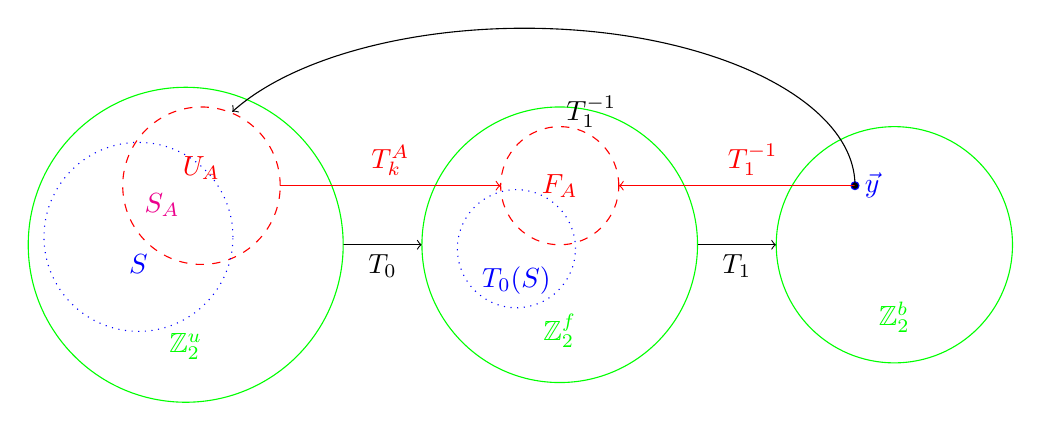
\begin{tikzpicture}
		\draw[->] (4,2) -- (5,2) node[left=0.5cm,below] {$T_0$};
		\draw[green] (2,2) circle (2cm) node[left=1cm,below=1cm] {$\binvecspace{u}$};
		\draw[green] (6.75,2) circle (1.75cm) node[left=0.75cm,below=0.75cm] {$\binvecspace{f}$};
		\draw[->] (8.5,2) -- (9.5,2) node[left=0.5cm,below] {$T_1$};
		\draw[green] (11,2) circle (1.5cm) node[left=0.6cm,below=0.6cm] {$\binvecspace{b}$};
		
		\draw[blue] (10.5,2.75) circle (0.05cm) [fill=black] node[anchor=west] {$\vec{y}$};
		\draw[->,red] (10.5,2.75) -- (7.5,2.75) node[left=-1.7cm,above] {$T_1^{-1}$};
		\draw[dashed,red] (6.75,2.75) circle (0.75cm)  node[] {$F_A$};
		\draw[dotted,blue] (6.2,1.95) circle (0.75cm)  node[left=0cm,below=0.1cm] {$T_0(S)$};

		\draw[dashed,red] (2.2,2.75) circle (1cm)  node[left=-0.35cm,below=-0.5cm] {$U_A$};
		\draw[dotted,blue] (1.4,2.1) circle (1.2cm)  node[left=0.35cm,below=0.1cm] {$S$};
		
		\draw[magenta] (1.7,2.5) node[] {$S_A$};
		

		\draw[->] (10.5,2.75) arc (0:152:4.2cm and 2cm) node[below=-1.5cm,left=-5cm] {$T_1^{-1}$};
		
		
		\draw[->,red] (3.2,2.75) -- (6,2.75) node[left=1.4cm,above] {$T_k^A$};
	\end{tikzpicture}
\end{center}
\end{figure}

\begin{figure}
	\caption{Factorisation of $T$ when event $E_2(S, T_0, T_1)$ occurs, i.e. $F_A \subseteq T_0(S)$.}
	\label{fig-factorisation-e2}

\begin{center}
	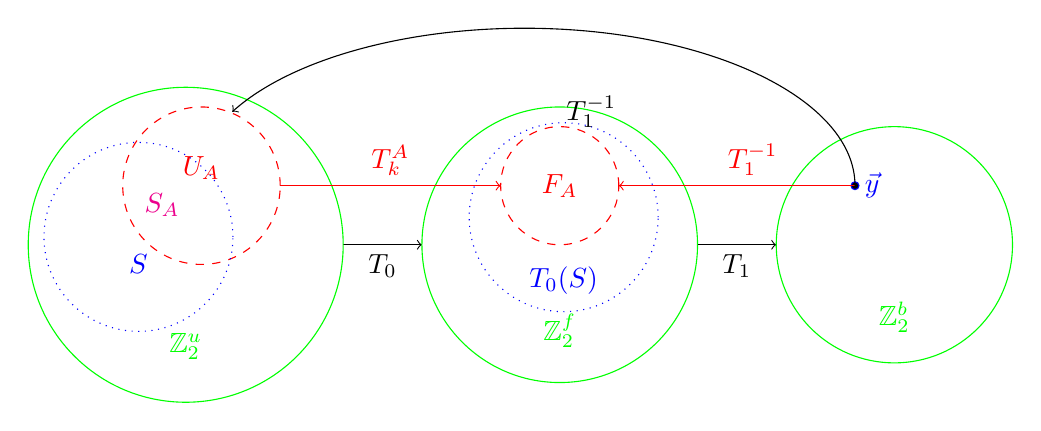
\begin{tikzpicture}
		\draw[->] (4,2) -- (5,2) node[left=0.5cm,below] {$T_0$};
		\draw[green] (2,2) circle (2cm) node[left=1cm,below=1cm] {$\binvecspace{u}$};
		\draw[green] (6.75,2) circle (1.75cm) node[left=0.75cm,below=0.75cm] {$\binvecspace{f}$};
		\draw[->] (8.5,2) -- (9.5,2) node[left=0.5cm,below] {$T_1$};
		\draw[green] (11,2) circle (1.5cm) node[left=0.6cm,below=0.6cm] {$\binvecspace{b}$};
		
		\draw[blue] (10.5,2.75) circle (0.05cm) [fill=black] node[anchor=west] {$\vec{y}$};
		\draw[->,red] (10.5,2.75) -- (7.5,2.75) node[left=-1.7cm,above] {$T_1^{-1}$};
		\draw[dashed,red] (6.75,2.75) circle (0.75cm) node[] {$F_A$};
		\draw[dotted,blue] (6.8,2.35) circle (1.2cm)  node[left=0cm,below=0.5cm] {$T_0(S)$};

		\draw[dashed,red] (2.2,2.75) circle (1cm)  node[left=-0.35cm,below=-0.5cm] {$U_A$};
		\draw[dotted,blue] (1.4,2.1) circle (1.2cm)  node[left=0.35cm,below=0.1cm] {$S$};

		\draw[->] (10.5,2.75) arc (0:152:4.2cm and 2cm) node[below=-1.5cm,left=-5cm] {$T_1^{-1}$};
		
		\draw[magenta] (1.7,2.5) node[] {$S_A$};
				
		\draw[->,red] (3.2,2.75) -- (6,2.75) node[left=1.4cm,above] {$T_k^A$};
	\end{tikzpicture}
\end{center}
\end{figure}

\begin{corollary}
\label{corollary-e1-e2}
For each $\epsilon > 0$ there is $c_\epsilon > 0$ such that if $l \geq c_\epsilon (f - b)2^{f-b}$, then
\[
\probs{T \in_U \linearmaps{u}{b}}{E_1(S, T, l)} \leq \frac{1}{1 - \epsilon}\probs{T_0 \in_U \linearmaps{u}{f}, T_1 \in_U \surjectivelinearmaps{f}{b}}{E_2(S, T_0, T_1)}
\]
\end{corollary}
\begin{proof}
\begin{claim}
\label{claim-dstr-affine}
Let $\vec{y} \in \binvecspace{b}$. For a fixed $T$ and $T_1$ the uniform choice of $T_0$ such that $T = T_0 \circ T_1$ gives the uniform choice of the affine linear mapping $T_k^A$ from $U_A$ to $F_A$ where $U_A = T^{-1}(\vec{y})$ and $F_A = T_1^{-1}(\vec{y})$.
\end{claim}
\begin{proof}
Proposition~3.4 in \cite{alonetal}.
\end{proof}
\begin{claim}
\label{claim-dstr-factor}
For a fixed onto linear mapping $T_1$ the uniform choice of $T_0$ gives the uniform choice of $T = T_0 \circ T_1$.
\end{claim}
\begin{proof}
See the beginning of the proof of \cref{theorem-epsilon} named Theorem~7a in \cite{alonetal}.
As a consequence notice that the uniform choice of $T$ is preserved even if $T_1$ is chosen randomly as well.
\end{proof}
From \cref{claim-dstr-affine} and \cref{lemma-e1-e2} it follows $1 - \epsilon \leq \probs{T_0, T_1}{E_2 | E_1}$ and directly from the definition of conditional probability we get $\probs{T_0, T_1}{E_1} \leq \frac{1}{1-\epsilon}\probs{T_0, T_1}{E_2}$.
Finally from \cref{claim-dstr-factor} it follows that $\probs{T}{E_1} = \probs{T_0, T_1}{E_1}$.
\end{proof}

Now we switch to estimating the probability of $E_2$. 
We start to differentiate from the original proof by choosing different size of the factor space.
The substantial change advantage is that we can start using the probability estimate coming from the following lemma for $f > b$ instead of $f > b + \log b$  from Proposition~3.1 of \cite{alonetal}.
On the other hand our estimate depends on $b$ and the calculation becomes a bit more complicated than the original one.

\begin{lemma}
\label{lemma-bound}
If $S \subseteq \binvecspace{u}$, $|S| = 2^b$ and $\mu = \frac{|S|}{|\binvecspace{f}|} = 2^{b - f} < 1$, then
\[
\probs{T_0 \in_U \linearmaps{u}{f}, T_1 \in_U \surjectivelinearmaps{f}{b}}{E_2(S, T_0, T_1)} \leq \mu ^ {-\log b - \log \mu + \log \log \mu^{-1}}.
\]
\end{lemma}
\begin{proof}
Observe that it is possible to restate $E_2(S, T_0, T_1)$ as $T_1(\binvecspace{f} - T_0(S)) \neq \binvecspace{b}$. 
Occurrence of $E_2(S, T_0, T_1) \equiv \exists \vec{y} \in \binvecspace{b} \colon T_1^{-1}(y) \subseteq T_0(S)$ is equivalent to $T_1(\binvecspace{f} - T_0(S))$ not containing $\vec{y}$, i.e. $E_2(S, T_0, T_1) \equiv \exists \vec{y} \colon \vec{y} \not\in T_1(\binvecspace{f} - T_0(S))$.
For more details of the situation check \cref{fig-factorisation-e2}.

We prove the estimate for arbitrary $T_0$ and thus it also holds for the uniform choice of $T_0$. 
We use \cref{theorem-prob-bound} to estimate $\probs{T_1\in_U \surjectivelinearmaps{f}{b}}{T_1(\binvecspace{f} - T_0(S)) \neq \binvecspace{b}} \leq \alpha ^ {f - b - \log b + \log \log \alpha^{-1}}$ where $\alpha = 1 - \frac{|\binvecspace{f} - T_0(S)|}{|\binvecspace{f}|} \leq \frac{|T_0(S)|}{2^f} \leq \frac{|S|}{2^f} \leq \mu$.
Since the function $\alpha ^ {f - b - \log b + \log \log \alpha^{-1}}$ is increasing w.r.t. $\alpha$ in $(0, 1)$ we get that
$
\probs{T_1 \in_U \surjectivelinearmaps{f}{b}}{E_2(S, T_0, T_1)} \leq \mu ^ {-\log \mu - \log b + \log \log \mu^{-1}}.
$
\end{proof} 

Now we compute the tail distribution of the variable $\lbin{T}{S}$ using the estimate from \cref{lemma-bound} which in turns directly gives \cref{theorem-n-to-n}.

\begin{theorem}
\label{theorem-prob-distribution-bound}
If $r > 4$, $\epsilon > 0$, then there is a constant $c_\epsilon > 0$ such that
\[
\probs{T \in_U \linearmaps{u}{b}}{\lbin{T}{S} \geq 2 c_\epsilon r} \leq \frac{1}{1 - \epsilon}\left(\frac{\log r}{r}\right)^{-\log b - \log \frac{\log r}{r} + \log \log \frac{r}{\log r}}.
\]
\end{theorem}
\begin{proof}
In this proof we fix $f = \lfloor b + \log r - \log \log r + 1 \rfloor$, $l = 2c_\epsilon r$ where $c_\epsilon$ comes from \cref{lemma-bound}.

As already mentioned in order to bound the probability of $E_1(S, T, l)$, i.e. $\lbin{T}{S} \geq l$, we first obtain an estimate on $\prob{E_2(S, T_0, T_1)}$ using the factorization through $\binvecspace{f}$. 

The choice of $f$ meets the requirement $f > b$ of \cref{lemma-bound} which also means that $\surjectivelinearmaps{f}{b}$ is nonempty.
To use \cref{corollary-e1-e2} we have to verify that $l \geq c_\epsilon (f - b)2^{f - b}$.
Since we assume that $r \geq 4$ we have $(f - b)2^{f - b} \leq (\log r - \log \log r + 1)2^{\log r - \log \log r + 1} \leq \frac{2r(\log r - \log \log r + 1)}{\log r} \leq 2r$ and this requirement is met.

Realize that $\mu = 2^{b - f} \leq \frac{\log r}{r}$ and that $f(\mu) = \mu ^ {- \log b + \log \mu^{-1} + \log \log \mu^{-1}}$ is increasing in $(0, 1)$.
From the previous facts and \cref{lemma-bound} we obtain that $\prob{E_2(S, T_0, T_1)} \leq f(\mu) \leq f(\log r/r)$.
\cref{corollary-e1-e2} directly implies the statement.
\end{proof}

When compared to the original proof the estimate from the proven theorem becomes less than one for $r \approx b$. 
This is possible because \cref{lemma-bound} may be used for smaller values of $f$ as was already mentioned.
The proof of the main theorem is now straightforward.

\begin{proof}[Proof of \cref{theorem-n-to-n}]
We fix $\epsilon > 0$ arbitrarily.
We split $\sum_{l = 1}^{n} \probs{T\in_U\linearmaps{u}{b}}{\lbin{T}{S} \geq l}$ into two sums according to $l$ being lower or greater than $8c_\epsilon \log n$.
In the second case we show that the probability of having a bin larger than $2 c_\epsilon r$ where $r \geq 4\log n$ is bounded from above by $\frac{r^{-1.5}}{1-\epsilon}$.
Hence $\sum_{l = 8c_\epsilon \log n}^{n} \probs{T\in_U\linearmaps{u}{b}}{\lbin{T}{S} \geq l} = \frac{O(1)}{1-\epsilon}$.
The first sum is estimated as $\sum_{l = 1}^{8c_\epsilon \log n} \probs{T\in_U\linearmaps{u}{b}}{\lbin{T}{S} \geq l} \leq 8c_\epsilon \log n$.

It remains to show that for $r \geq 4 \log n$ the estimate obtained by \cref{theorem-prob-distribution-bound} is below $\frac{r^{-1.5}}{1-\epsilon}$.
To do so we bound the exponent coming from the theorem from below.
\[
-\log b - \log \log r + \log r + \log (\log r - \log \log r) \geq -\log \log r + 2 + \log \left(\frac{3\log r}{4}\right) = \log(3).
\]
Hence for $r \geq 4\log n$ we may conclude that $\prob{\lbin{T}{S} \geq 2c_\epsilon r} \leq \frac{\left(\frac{\log r}{r}\right)^{\log 3}}{1-\epsilon} \leq \frac{r^{-1.5}}{1-\epsilon}$.
\end{proof}

\section{The special case when balls form a vector subspace}
\todo{This is a redundent section possibly.}

Let us note that when $S$ is a subspace of the universe, then the expected size of the largest bin is constant.

\begin{theorem}
Let $b, u \in \mathbb{N}$ and $v_1, \dots, v_b \in \mathbb{Z}_2^u$ be linearly independent. Then \[ \expects{h \in_U \linearmaps{u}{b}}{\lbin{h}{\operatorname{Span}(v_1, \dots, v_b)}} = O(1) .\]
\end{theorem}
\begin{proof}
We first notice that the bins have a simple structure -- all of them are formed by elements which are affine subspaces of the universe.
This means that the non-empty bins have the same size.
In addition the bin $\vec{0}$ in $\binvecspace{b}$ is always non-empty is a largest bin of expected constant size.

For convenience put $S = \operatorname{Span}(v_1, \dots, v_b)$. 
We show that each non-empty bin created by a transformation $h$ is formed by balls from an affine subspace of $S$ and has the size of the kernel of $h$.
From this it follows that $\expect{\lbin{h}{S}} = \expect{\bin{h}{S}{0}} = O(1)$.

Without loss of generality assume that $v_1, \dots, v_k$ are the vectors forming the kernel of $h$, i.e. $h(v_i) = 0$ where $i \in \{1, \dots, k\}$.
If $h(v) = y$ for some $v \in S$, then $h^{-1}(y) \cap S = v + \operatorname{Span}(v_1, \dots, v_k)$.
Hence for each $y \in \mathbb{Z}_2^b$ it holds hat $|h^{-1}(y) \cap S| = 0 \vee |h^{-1}(y) \cap S| = 2^k$.
Thus the sizes of all the non-empty bins are the same and are equal to $\bin{h}{S}{0}$.
\end{proof}

\section{Acknowledgement}

We would like to thank V\'aclav Koubek and Michal Kouck\'y for many advices, consultations and time spent verifying the result. \todo{Venovanie Vaskovi - ale co napisat?}

\bibliographystyle{siamplain}
\bibliography{lhf}

\end{document}
